%%%%%%%%%%%%%
\chapter{Evaluation}
\label{ch:evaluation}
%%%%%%%%%%%%%

Nach der Durchführung der Studie gilt es, die Ergebnisse dieser auszuwerten und einzuordnen. Hierfür werden mehrere erhobenen Daten betrachtet. Die Evaluation der Studienergebnisse besteht zunächst aus der Beschreibung der Charakteristika der Probandengruppe. Anschließend werden die Ergebnisse der Erhebungen beschrieben. Eingegangen wird hierbei auf die Ergebnisse der Fragebögen, sowie der Abschließenden Fragerunde. Abschließend werden die Ergebnisse der Fragebögen mit den Einschätzungen der Fragerunde in Verbindung gebracht. 


\section{Deskriptive Statistik}
Es nahmen acht Probanden an der Vergleichsstudie teil. Diese befinden sich zum Zeitpunkt der Durchführung im Alter von 23 bis 37 Jahren. Das durchschnittliche Alter beträgt 29. Die Probandengruppe setzt sich aus fünf Frauen und 3 Männern zusammen. Die Probanden sind wissenschaftliche Mitarbeiter, Promotionsstudenten oder Doktoren aus dem medizinischen Bereich. 

Folgende Aussagen lassen sich über die Gewohnheiten und Technologienutzung der Probanden ableiten. Die Mehrheit verwendet ein- oder mehrmals am Tag Chat-Technologien. Ein Proband nutzt Chat-Technologien 
einmal im Monat oder seltener. Die verwendeten Chat-Technologien setzen sich aus Whatsapp, Telegram, Facebook Messenger, Instagram, Threema, Apple Nachrichten, Line und Slack zusammen. Die meistgenutzten Chat-Technologien innerhalb der Probandengruppe sind Whatsapp und Facebook Messenger. Verwendet werden diese Anwendungen hauptsächlich auf dem Smartphone oder Laptop bzw. Desktop Computer. 

Die Nutzung von Chatbots ist innerhalb der Probandengruppe wenig verbreitet. Diese werden von zwei Probanden einige Male pro Woche und einmal im Monat oder weniger genutzt. Genutzt werden der Nachrichtenbot der Tagesschau und ein Chatbotdienst für den Kundenservice der Firma ASOS. Bedient werden diese Chatbotdienste auf dem Smartphone sowie Laptop bzw. Desktop Computer. 

Innerhalb der Probandengruppe wurde Experience Sampling bereits mehrheitlich genutzt. Drei Probanden gaben an noch nie oder nur gelegentlich Experience Sampling verwendet zu haben. Fünf Probanden haben bereits Experience Sampling öfters bis regelmäßig genutzt. Für Experience Sampling kamen die Anwendungen MovisensXS, Menthal und Whatsanalyzer zum Einsatz. Genutzt wurden diese auf dem Smartphone oder Laptop bzw. Desktop Computer. 

Hinsichtlich der Vorerfahrungen bezüglich MovisensXS lassen sich für die Probandengruppe folgende Aussagen treffen. Wie in Grafik \ref{movisensXSErfahrung} zu sehen ist, besitzt ein Proband keinerlei Erfahrungen mit MovisensXS. Die restlichen Probanden nutzen das Programm gelegentlich bis regelmäßig. Die Nutzung von MovisensXS beschränkt sich auf das Zuordnen von Probanden, Teilnahme an Studien, sowie kleinen Anpassungen einer bereits bestehenden Studie. 

\begin{figure}[h]
\centering
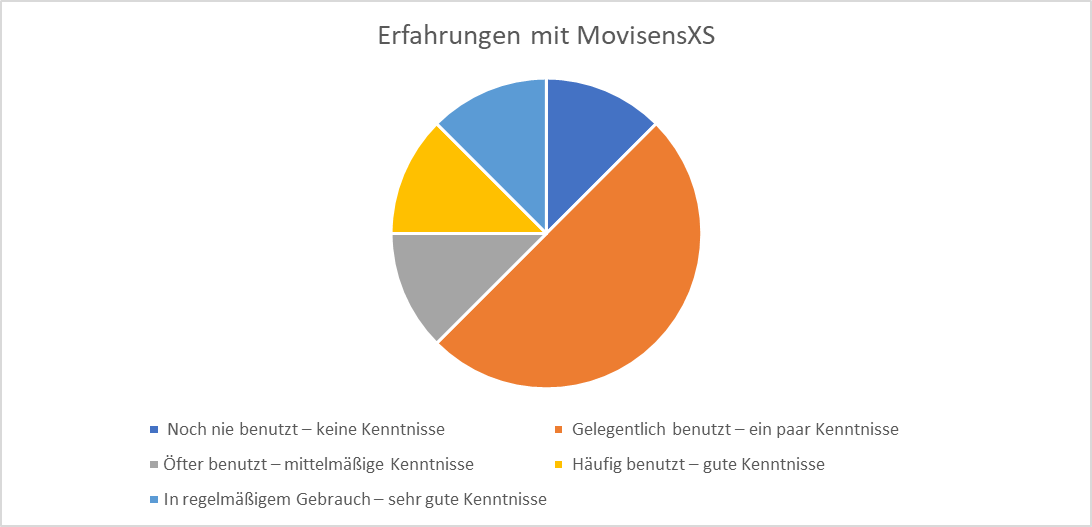
\includegraphics[width=1\textwidth]{pictures/diagramme/movi}
\caption{Angaben der Probanden bezüglich ihrer Erfahrungen mit dem Programm \emph{MovisensXS}}
\label{movisensXSErfahrung}
\end{figure}

Basierend auf dieser Probandengruppe ist es für die Überprüfung der aufgestellten Hypothesen bedeutend, die jeweiligen Probanden zu framen. Hierfür werden zunächst Sinn der Studie und diverse Begriffe erläutert. Anschließend machen sich die Probanden zunächst mit dem jeweiligen Programm vertraut, welches betrachtet werden soll. Hierfür wird eine Aufgabe gestellt, die durch das Programm führt und den Probanden beim explorieren des jeweiligen Programms und dessen Funktionen anleitet. Während der Nutzung und der Bearbeitung der gestellten Aufgaben, werden Emotionen und Motivationen durch Kommentare des Probanden erfasst. Abschließend wird nach der aufgabengesteuerten Nutzung eines Programms eine erste Einschätzung in Form eines Fragebogens erfasst. Nach Bearbeitung aller Aufgaben und Verwendung beider Programme, werden die Programme in einer abschließenden Fragerunde miteinander verglichen. Dabei wird auf wesentliche Unterschiede beider Programme eingegangen. Erfasst werden hierbei die Einschätzung der Probanden, welche Eigenschaften sie im Vergleich als besonders Hilfreich, nicht Hilfreich empfanden. Auch welche Eigenschaften ihnen gefallen oder welche sie vermisst haben. Diese Einschätzungen werden in Relation zu den Ergebnissen der Fragebögen gesetzt um diese zu verargumentieren.


\section{Beschreibung der Ergebnisse}

Zunächst werden die Ergebnisse der Fragebögen betrachtet. Diese werden in verschiedene Kategorien eingeordnet, in denen sich die Ansätze maßgeblich unterscheiden. Die Einschätzungen der abschließenden Fragerunde der Studie werden ebenfalls betrachtet. Abschließend werden die Ergebnisse verknüpft und im Kontext der aufgestellten Hypothesen diskutiert. 

\subsection{Konstruktionsprinzip versus Konfigurationsprinzip}

Die Programme \emph{TherapyBuilder} und \emph{MovisensXS}, der Studie, unterscheiden sich maßgeblich in der Herangehensweise der Einstellung der Trigger. Während \emph{TherapyBuilder} das Konfigurationsprinzip verfolgt, nutzt \emph{MovisensXS} das Konstruktuionsprinzip. Die Studienergebnisse beider Ansätze werden zunächst getrennt betrachtet. Für diese Betrachtung werden vorerst die Ergebnisse der Fragebögen herangezogen. Abschließend erfolgt die Gegenüberstellung beider Ansätze. 

\subsubsection{Ergebnisbeschreibung des Konstruktionsprinzips}

Das Konstruktionsprinzip bietet das Einstellen der Trigger durch das Zusammensetzen und Verschalten einzelner Blöcke mit unterschiedlichen Funktionen. Wie in Abbildung \ref{konstruktion} dargestellt, bildet sich aus der Anordnung ein Baum aus verschiedenen Blöcken. Die Blöcke unterscheiden sich farblich und folgen dem Ampelprinzip.  

\begin{figure}[h]
\centering
\includegraphics[width=1\textwidth]{pictures/konstruktion}
\caption{Das Konstruktionsprinzip des MovisensXS. Blöcke werden miteinander verschaltet.}
\label{konstruktion}
\end{figure}

Die Probanden gaben nach der Aufgabenbearbeitung an, dass sie die Darstellung der Trigger als zumeist schon verständlich empfanden mit einer leichten Tendenz zu zum Teil verständlich. Dies wird auch durch die Freitext-Aussagen der Probanden gestützt. Fünfundsiebzig Prozent der Probanden gingen auf die positive Auswirkung der farblichen Kodierung. Zum einen wurde beschrieben, dass diese die Orientierung innerhalb des Baumes erleichtern und die Funktion sowie Abfolge der Bausteine gut beschreiben.

Die Verständlichkeit der Einstellungsmöglichkeiten wurde von den Probanden sehr unterschiedlich bewertet. Im Schnitt wird diese als zum Teil verständlich und zumeist schon verständlich empfunden. 



\subsubsection{Ergebnisbeschreibung des Konfigurationsprinzip}

\begin{figure}[h]
\centering
\includegraphics[width=1\textwidth]{pictures/konfiguration}
\caption{Architektur des \emph{konfiguration}}
\label{konfiguration}
\end{figure}


\subsubsection{Gegenüberstellung}

\begin{figure}[h]
\centering
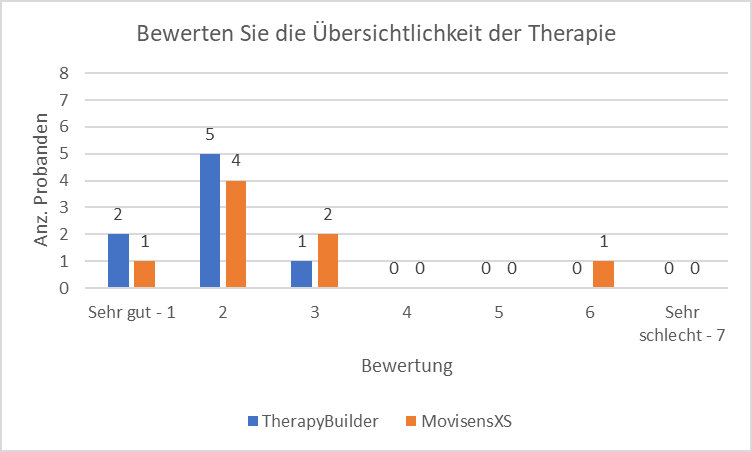
\includegraphics[width=1\textwidth]{pictures/diagramme/therapieuebersicht}
\caption{Architektur des \emph{konfiguration}}
\label{therapieuebersicht}
\end{figure}

\begin{figure}[h]
\centering
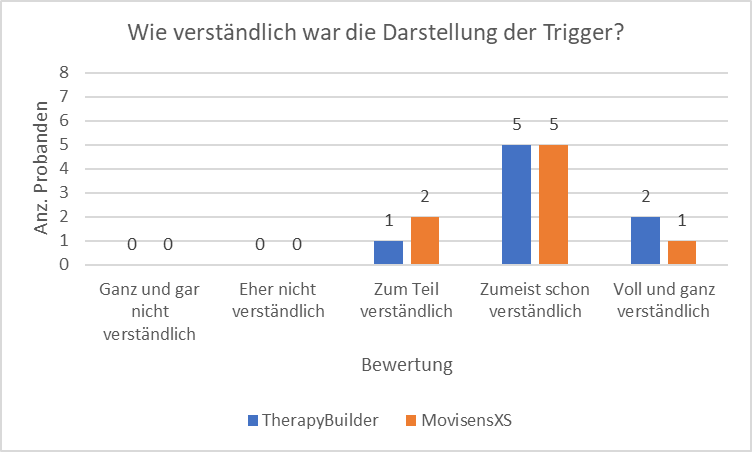
\includegraphics[width=1\textwidth]{pictures/diagramme/triggerdarstellung}
\caption{Architektur des \emph{konfiguration}}
\label{triggerdarstellung}
\end{figure}

\begin{figure}[h]
\centering
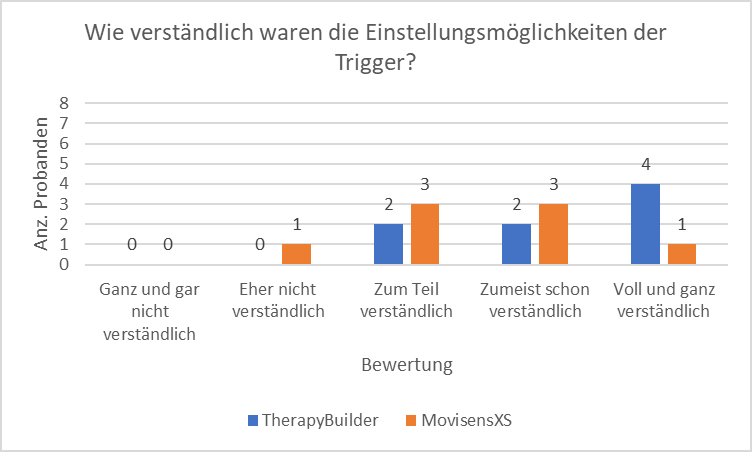
\includegraphics[width=1\textwidth]{pictures/diagramme/triggereinstellung}
\caption{Architektur des \emph{konfiguration}}
\label{triggereinstellung}
\end{figure}

\begin{figure}[h]
\centering
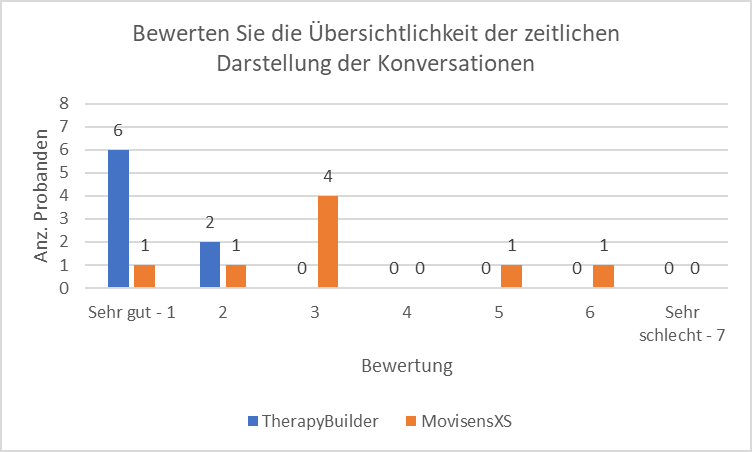
\includegraphics[width=1\textwidth]{pictures/diagramme/konversationzeitldarstellung}
\caption{Architektur des \emph{konfiguration}}
\label{konversationzeitldarstellung}
\end{figure}

\begin{figure}[h]
\centering
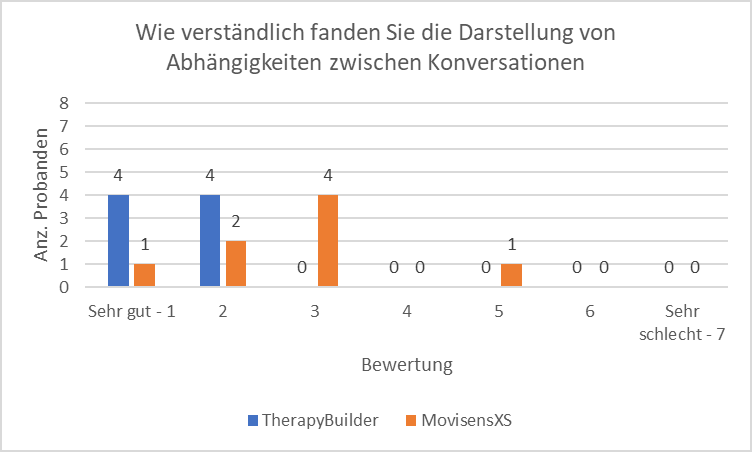
\includegraphics[width=1\textwidth]{pictures/diagramme/konversationenabhaeng}
\caption{Architektur des \emph{konfiguration}}
\label{konversationenabhaeng}
\end{figure}

\begin{figure}[h]
\centering
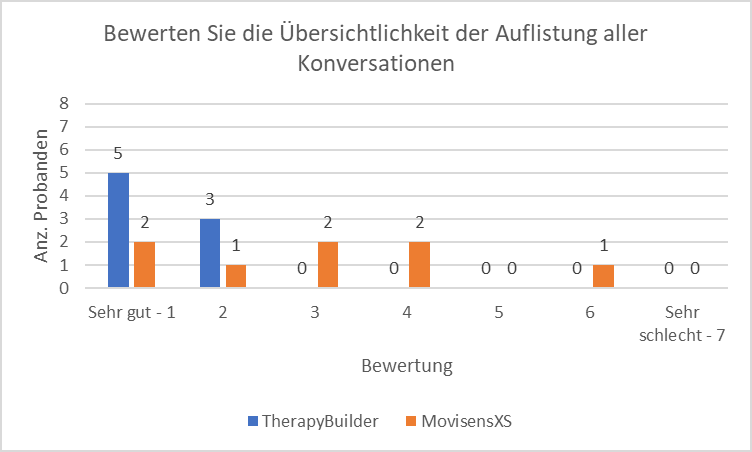
\includegraphics[width=1\textwidth]{pictures/diagramme/konversationenuebersicht}
\caption{Architektur des \emph{konfiguration}}
\label{konversationenuebersicht}
\end{figure}

\begin{figure}[h]
\centering
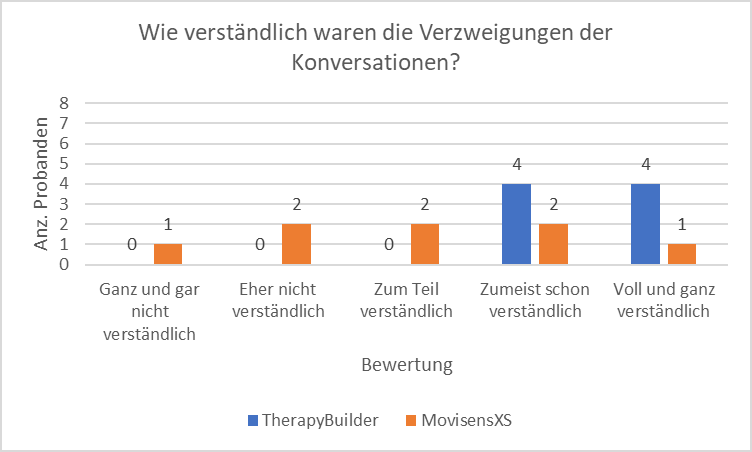
\includegraphics[width=1\textwidth]{pictures/diagramme/konversationverzweigung}
\caption{Architektur des \emph{konfiguration}}
\label{konversationverzweigung}
\end{figure}



\subsection{Sprünge versus Sichtbarkeitsregeln}

\subsubsection{Sprünge}

\begin{figure}[h]
\centering
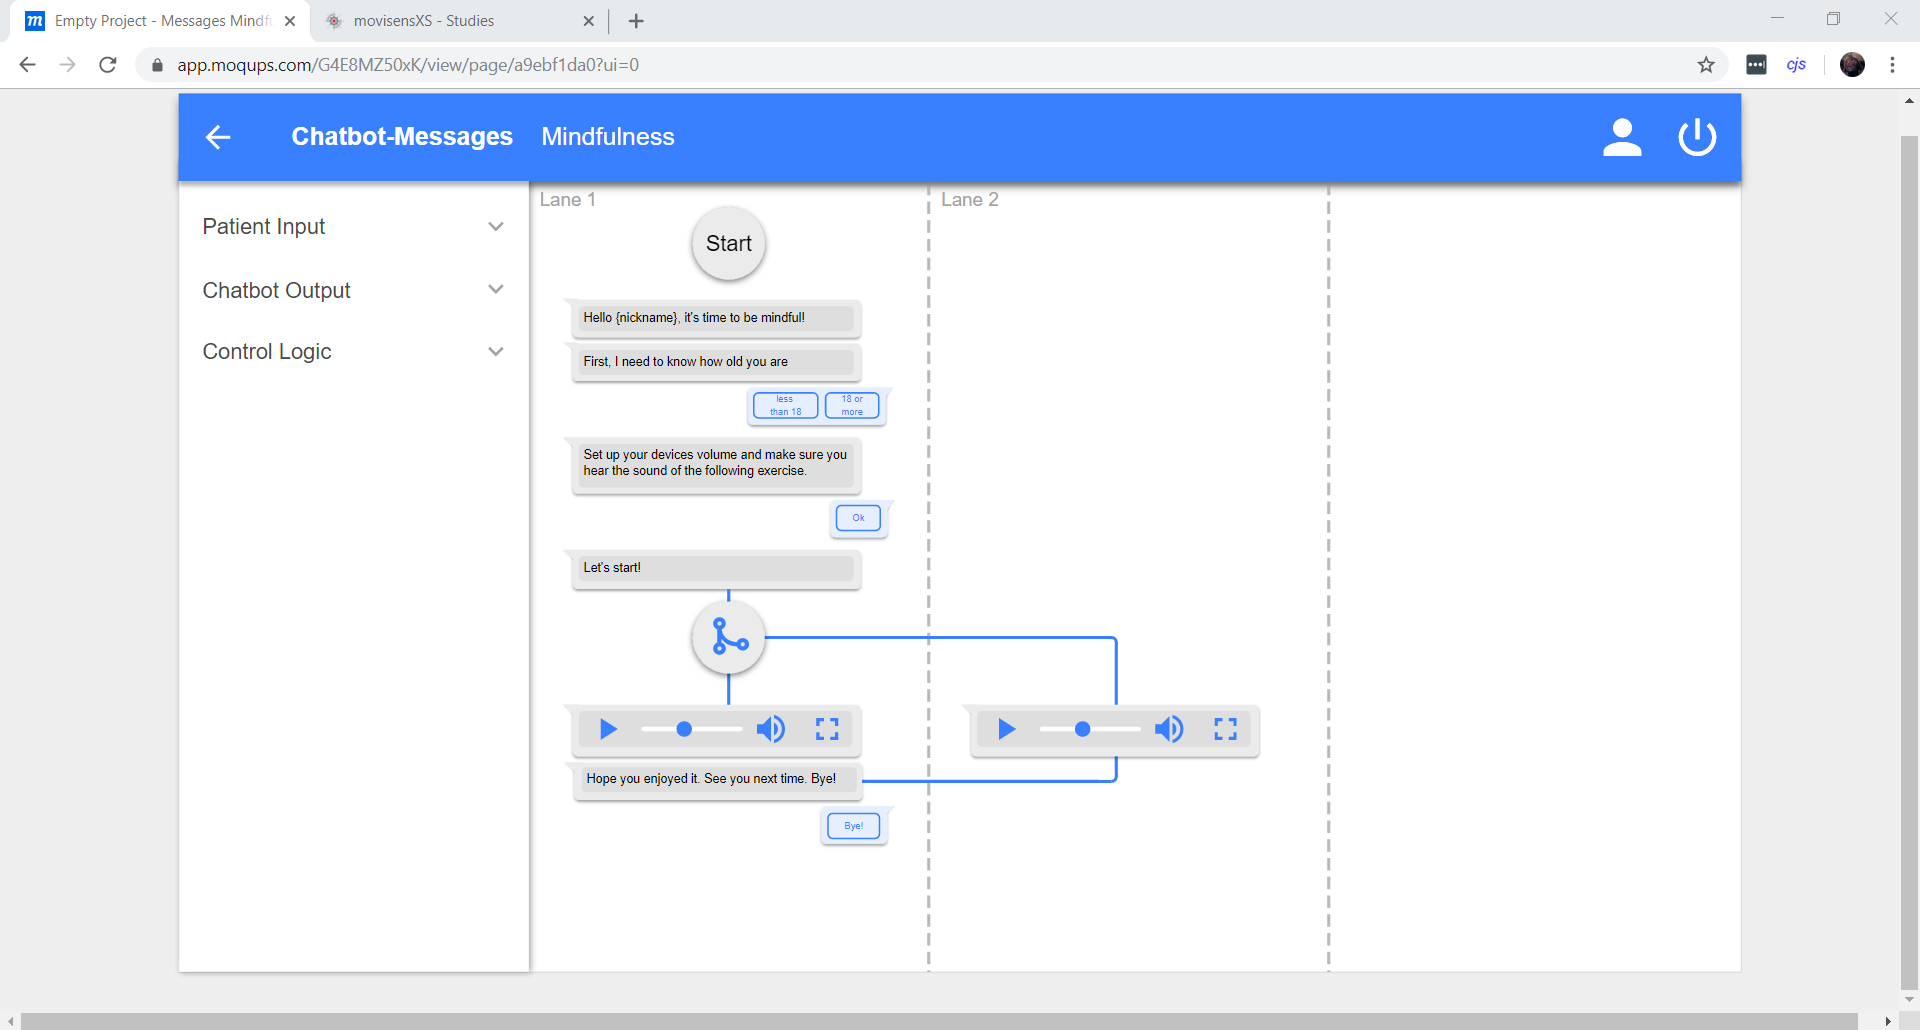
\includegraphics[width=1\textwidth]{pictures/spruenge}
\caption{Architektur des \emph{spruenge}}
\label{spruenge}
\end{figure}


\subsubsection{Sichtbarkeitsregeln}

\begin{figure}[h]
\centering
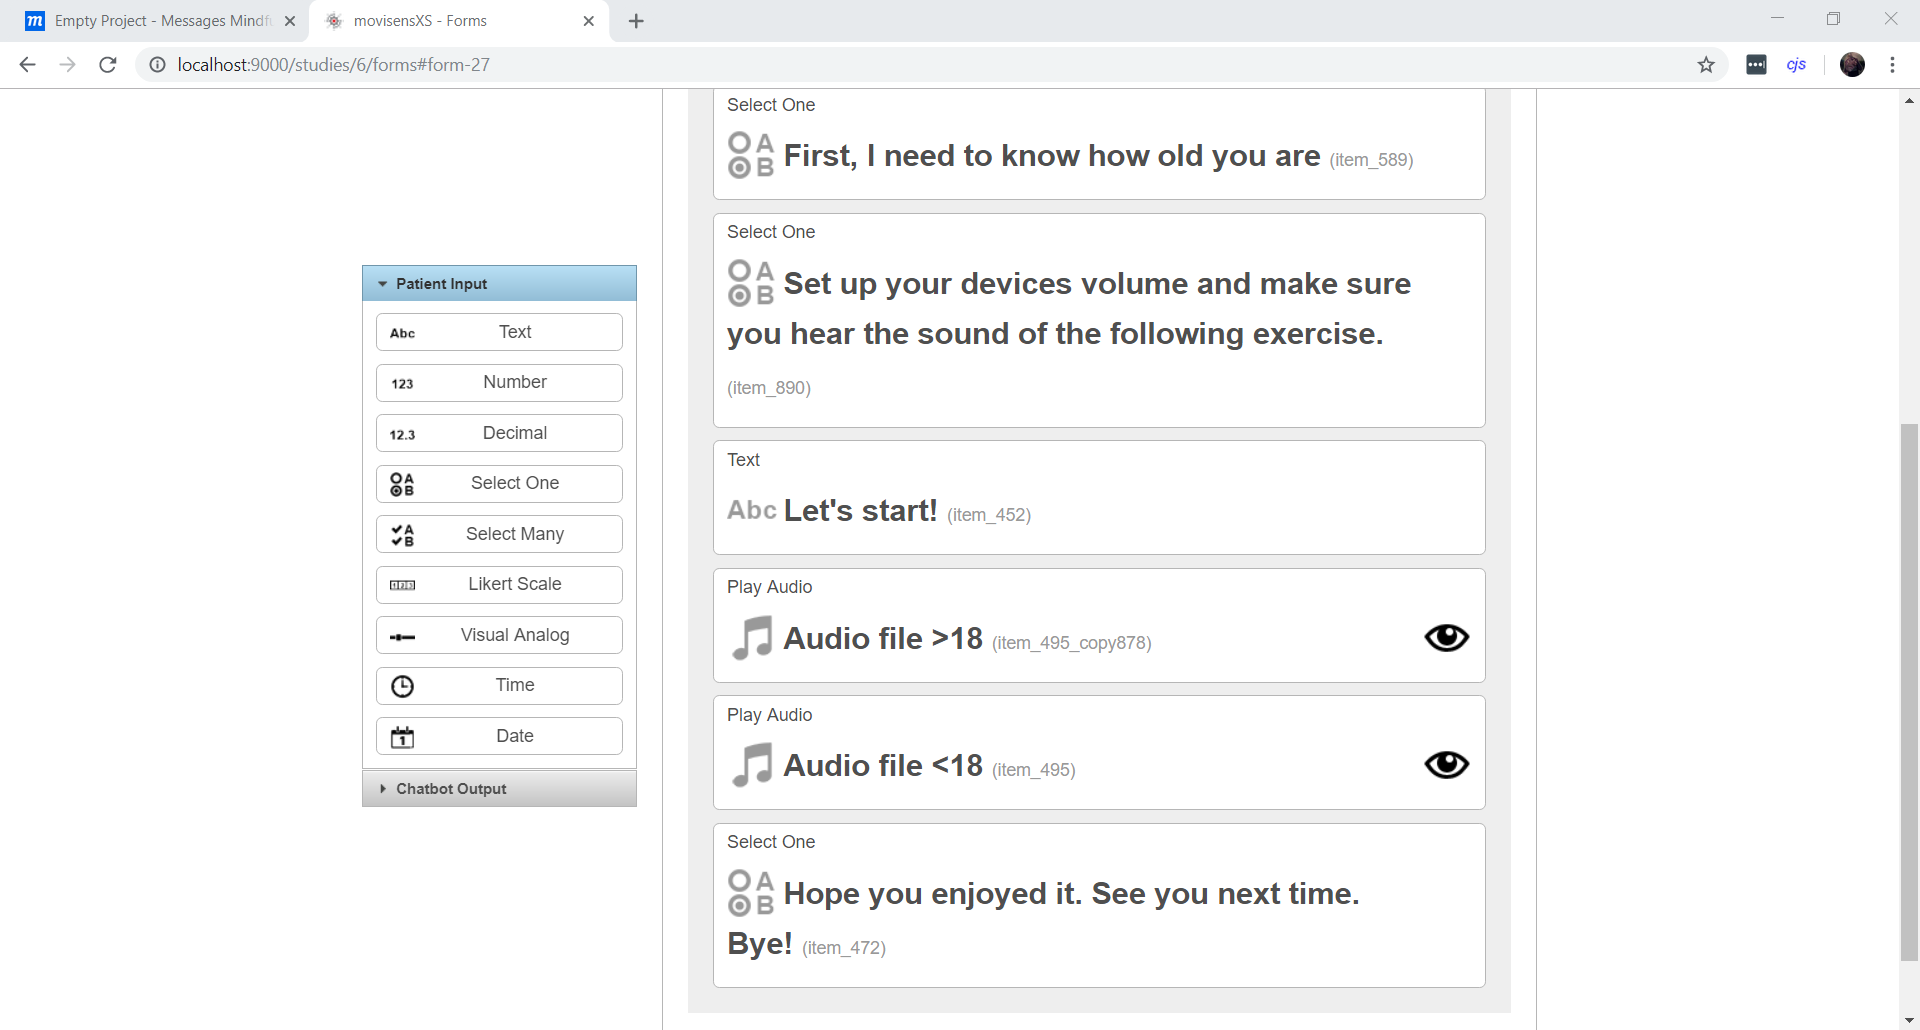
\includegraphics[width=1\textwidth]{pictures/sichtbarkeit}
\caption{Architektur des \emph{sichtbarkeit}}
\label{sichtbarkeit}
\end{figure}


\subsubsection{Gegenüberstellung}

\begin{figure}[h]
\centering
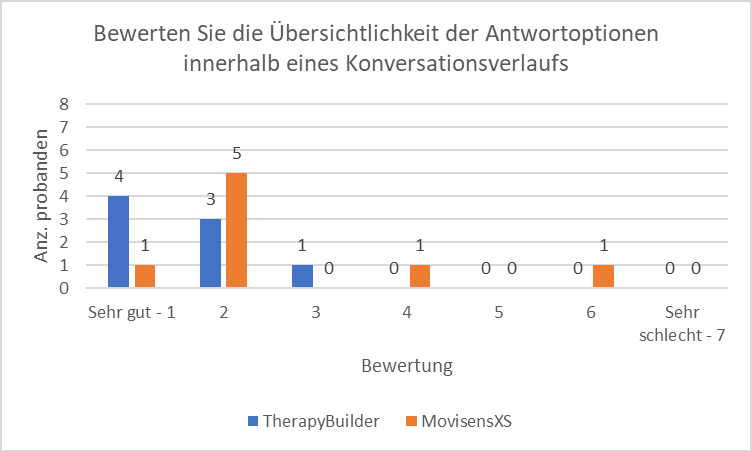
\includegraphics[width=1\textwidth]{pictures/diagramme/antwortoptkonv}
\caption{Architektur des \emph{sichtbarkeit}}
\label{antwortoptkonv}
\end{figure}

\begin{figure}[h]
\centering
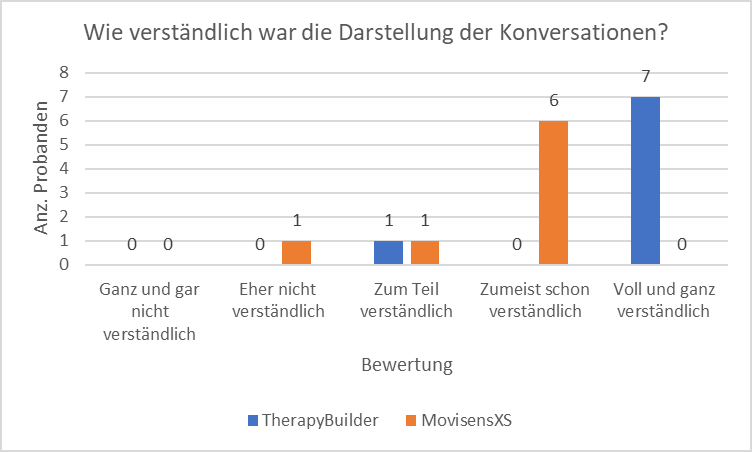
\includegraphics[width=1\textwidth]{pictures/diagramme/konversationdarstellung}
\caption{Architektur des \emph{konfiguration}}
\label{konversationdarstellung}
\end{figure}

\begin{figure}[h]
\centering
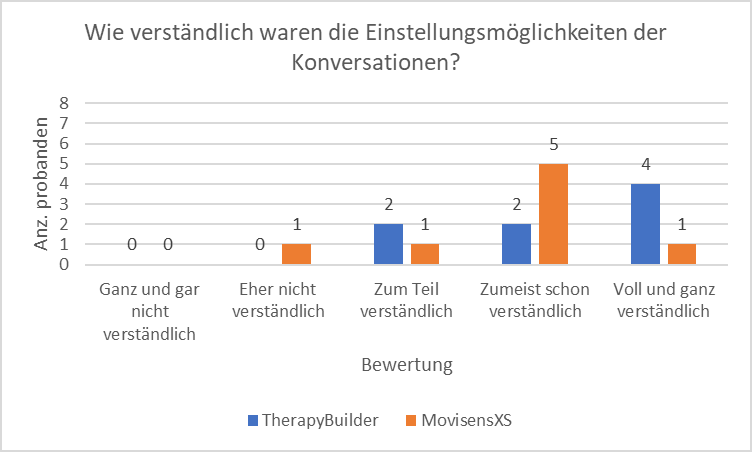
\includegraphics[width=1\textwidth]{pictures/diagramme/konversationeinstellung}
\caption{Architektur des \emph{konfiguration}}
\label{konversationeinstellung}
\end{figure}



\begin{figure}[h]
\centering
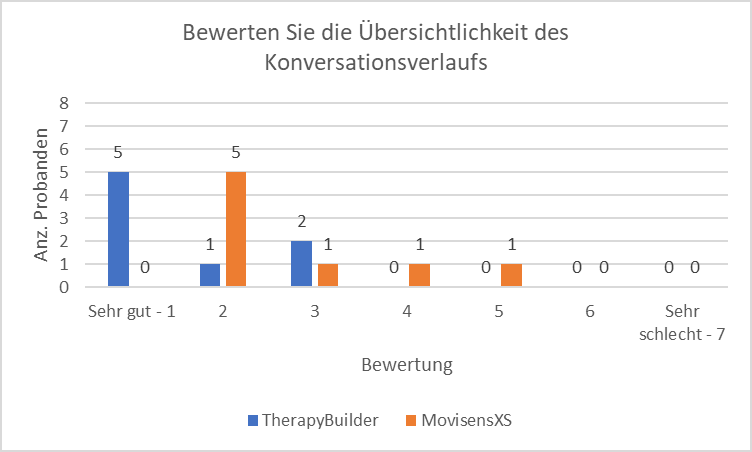
\includegraphics[width=1\textwidth]{pictures/diagramme/konversationverlfueber}
\caption{Architektur des \emph{konfiguration}}
\label{konversationverlfueber}
\end{figure}

\begin{figure}[h]
\centering
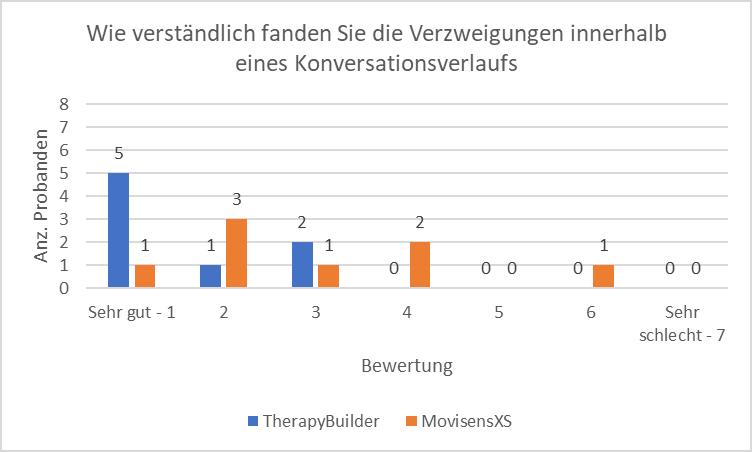
\includegraphics[width=1\textwidth]{pictures/diagramme/konvverzweig}
\caption{Architektur des \emph{konfiguration}}
\label{konvverzweig}
\end{figure}


\begin{figure}[h]
\centering
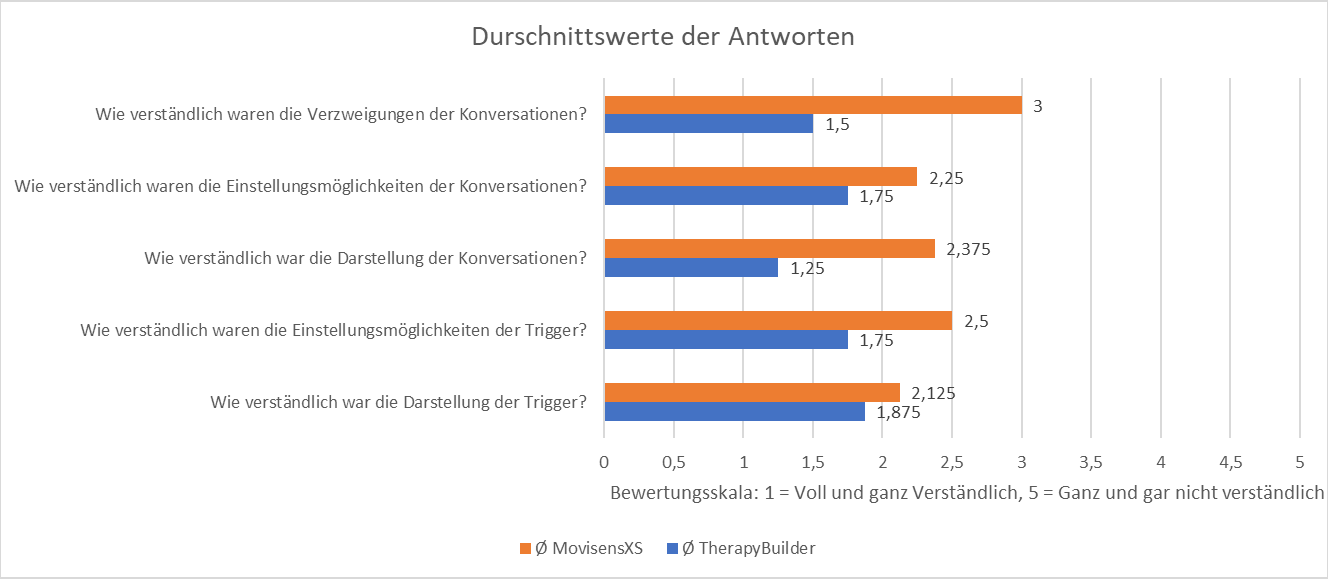
\includegraphics[width=1\textwidth]{pictures/diagramme/antwortendurchsch1}
\caption{Architektur des \emph{konfiguration}}
\label{antwortendurchsch1}
\end{figure}

\begin{figure}[h]
\centering
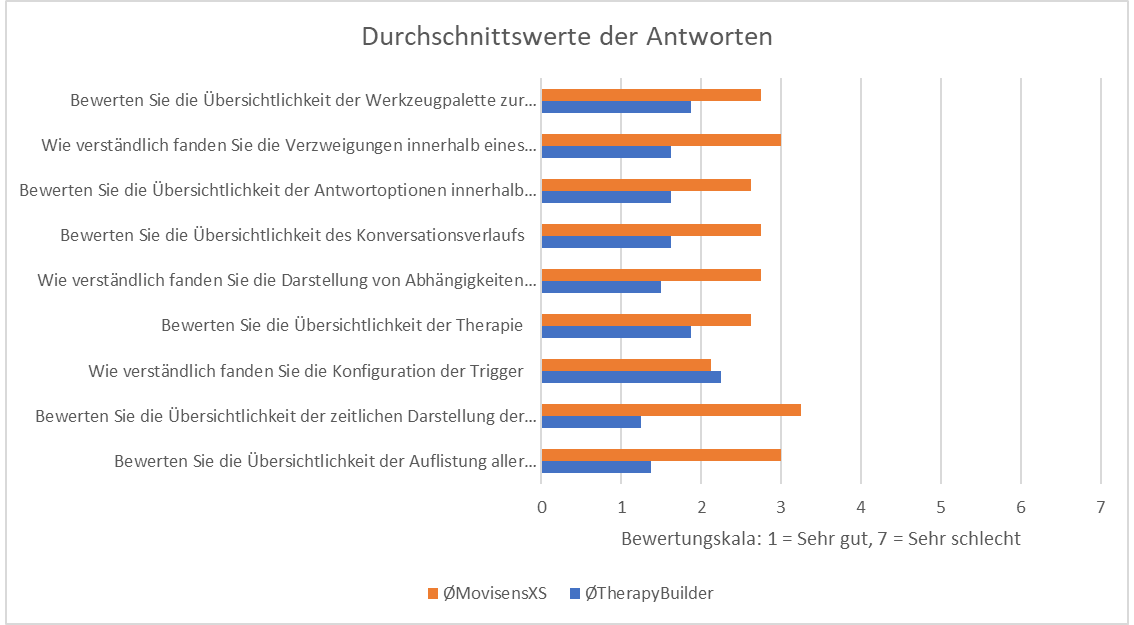
\includegraphics[width=1\textwidth]{pictures/diagramme/antwortendurchsch2}
\caption{Architektur des \emph{konfiguration}}
\label{antwortendurchsch2}
\end{figure}

